% -*-coding: utf-8;-*-
%\section{Описание программного пакета}

\subsection{Основные решаемые задачи}

В соответствии со своим назначением программный пакет должен решать
задачи моделирования САУ, моделирования и обучения нейронных сетей.
Типовой сеанс работы с пакетом подразумевает интерактивное
взаимодействие пользователя с программами.  Поскольку пакет
разрабатывается для применения в учебном процессе, весьма желательно,
чтобы он был:
\begin{itemize}
\item простым в изучении и использовании;
\item адаптированным к специфике учебного процесса;
\item быстродействующим на не самых современных компьютерах;
\item открытым к модификации;
\item основанным на общедоступных и открытых технологиях.
\end{itemize}

При моделировании систем автоматического управления необходимо
предусмотреть возможность гибкой настройки контура и условий его
работы.  В частности, должны настраиваться:
\begin{itemize}
\item уставка (стохастическая, детерминированная);
\item помеха (стохастическая, детерминированная);
\item регулятор (линейный, нейросетевой);
\item объект управления (линейный, нелинейный, нестационарный).
\end{itemize}

%TODO: аргументировать, почему эти свойства важны.  м.б., в первой главе

В то же время, учитывая учебную направленность пакета, представляется
достаточным ограничиться одномерными системами управления когда объект
является одноканальным по входу и выходу.  Это существенно упрощает
интерактивную часть пакета и практику его использования.

Для моделирования и обучения нейронных сетей должны иметься следующие
возможности:
\begin{itemize}
\item создание нейронной сети с произвольной архитектурой в классе
  многослойных персептронов;
\item обучение нейронной сети на обучающей выборке с контролем
  процесса по тестовой выборке;
\item предсказание поведения объекта управления с помощью нейронной
  сети в контуре в процессе моделирования;
\item обучение нейронной сети регулятора в контуре управления в
  процессе его моделирования.
\end{itemize}

Специфика применения нейронных сетей в системах автоматического
управления заключается в преимущественном использовании сетей класса
``многослойный персептрон'' с обучением методом обратного
распространения или более эффективными его вариантами.  По этой
причине нецелесообразно реализовывать поддержку сетей существенно иных
парадигм (Кохонена, Хопфилда и пр.).  Иногда применяемые в САУ
нейронные сети, основанные на радиально-базисных функциях (RBF),
доказанно являются эквивалентными многослойному персептрону, поэтому
их реализация тоже является избыточной и ради простоты программного
комплекса от неё целесообразно отказаться.

\subsection{Структура пакета и выбор инструментария}

Анализ требований к пакету обнаруживает, что некоторые из них трудно
совместить, пользуясь какой-то одной инструментальной технологией
разработки программ.  В частности, эффективное выполнение
вычислительных алгоритмов требует компиляции программ перед
выполнением.  Только с помощью компиляции можно обеспечить приемлемое
быстродействие на не всегда современных компьютерах, используемых в
учебном процессе.  В то же время, открытость к модификации
подразумевает возможность изменения программы прямо перед выполнением,
что важно для быстрой разработки, а также при углубленном изучении
пакета программ и проведении исследований с его помощью.

Кроме того, не все технологии разработки программного обеспечения
доступны на всех распространенных операционных системах: Microsoft
Windows, Linux, Mac OS X.  Некоторые из подходящих технологий
реализованы только в проприетарных программных продуктах,
использование которых требует покупки дорогостоящей лицензии.

В \tablref{tabl:sdk_tech} приводятся данные о сравнении нескольких
различных современных технологий разработки программного обеспечения
по перечисленным трем критериям.  Под технологиями в данном случае
понимается совокупность языка программирования, среды разработки и
выполнения и необходимые средства для реализации пользовательского
интерфейса и интерактивной графики.

\begin{table}[ht]
\centering
\caption{Сравнение технологий разработки программ.}
\label{tabl:sdk_tech}
\begin{tabular}{|l|c|c|c|}
\hline
\bf Технология & \bf Быстродействие & \bf Открытость к & \bf Общедоступность \\
             &                & \bf модификации  & \bf и открытость \\
\hline
             &                &  плохо       &              \\
\tt C++      &   отлично      & (требуется   & отлично      \\
             &                & компиляция)  &              \\
\hline
             &   средне       &  плохо       &              \\
\tt Java     & (интерпретация & (требуется   & отлично      \\
             & байт-кода)     & компиляция)  &              \\
\hline
             &   средне       &  плохо       & плохо        \\
\tt C$\#$    & (нужно много   & (требуется   & (в основном, \\
             & ресурсов)      & компиляция)  & для MS Windows) \\
\hline
            &   плохо        &              & средне       \\
\tt Python  & (интерпретация & отлично      & (нет единого \\
            & байт-кода)     &              & подхода к GUI) \\
\hline
           &   плохо        &              &              \\
\tt Tcl/Tk & (интерпретация & отлично      & отлично      \\
           & байт-кода)     &              &              \\
\hline
           &   средне       &              & плохо        \\
\tt Matlab & (интерпретация & отлично      & (платный и   \\
           & байт-кода)     &              & очень дорогой) \\
\hline
\end{tabular}
\end{table}

Отсутствие идеальной технологии для разработки пакета моделирования и
нейросетевого управления вынуждает искать компромиссное решение.
Можно функционально разделить пакет на интерактивную и вычислительную
части и реализовать каждую с помощью оптимальной технологии.
Вычислительная часть требует эффективной реализации с точки зрения
быстродействия, поэтому целесообразно реализовать её на языке {\tt
  C++}.  Компиляторы этого языка программирования доступны для всех
значимых платформ, а сам язык, пожалуй, является в настоящее время
наиболее популярным среди универсальных процедурных языков
программирования.

Интерактивную графику и управление вычислительными алгоритмами важно
сделать максимально гибкими и открытыми для модификации.  Хорошим
выбором будет использование интерпретируемого языка с встроенными
возможностями для реализации пользовательского интерфейса, прикладной
графики и средствами интеграции программного обеспечения.  Одним из
подходящих инструментов является {\tt Tcl/Tk}, доступный бесплатно и в
исходных текстах для всех распространенных операционных систем.

Функциональная декомпозиция разрабатываемого пакета по используемым
технологиям разработки программ находит отражение в структуре
взаимодействия отдельных частей программного комплекса, которая
приводится на \figref{fig:prog_interaction_struct}.  Реализация
вычислительных функций в отдельных узко-специализированных программах,
написанных на языке {\tt C++}, позволит пользователю гибко управлять
их взаимодействием и во многих нестандартных случаях снизит
необходимость в модификации текстов на {\tt C++}.

\begin{figure}
\centerline{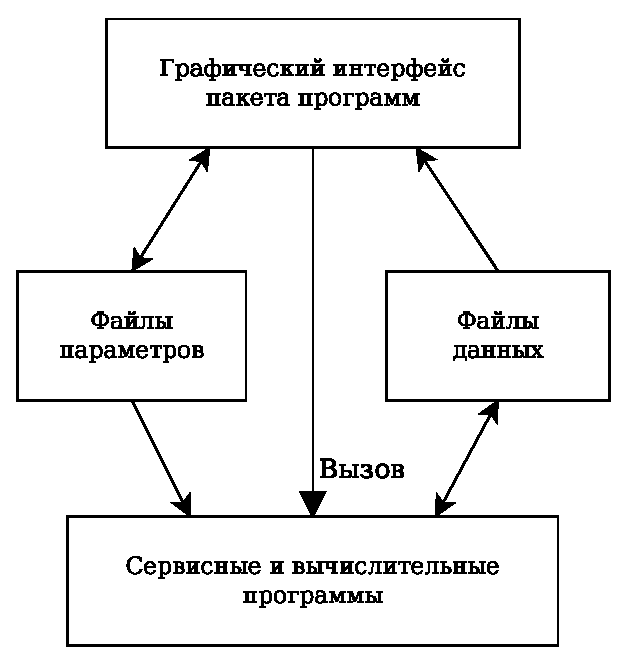
\includegraphics{princ_struct.eps}}
\caption{Схема взаимодействия частей программного пакета}
\label{fig:prog_interaction_struct}
\end{figure}

\subsection{Основные интерактивные элементы}
\subsection{Вспомогательные интерактивные элементы}
\subsection{Сервисные и вычислительные программы}


\subsection{Объектная библиотека}
\subsubsection{Абстракции данных и вспомогательный сервис}
\subsubsection{Ввод-вывод, параметры}
\subsubsection{Функциональные блоки от {\tt NaUnit} (+ .tf, .cof, .nn)}
\subsubsection{Нейросетевые элементы, методы обучения}
\subsubsection{Базовые объекты для построения сетей Петри}
\subsubsection{Объекты для моделирования дискретных динамических систем}
\subsubsection{Формализм для графического представления динамических моделей}
\subsubsection{Пример: дообучение нейросетевого регулятора в контуре}
\subsubsection{Пример: моделирование САУ и обнаружение разладки}
